\chapter{Rectangular Beams}
\section{Introduction}Ductile reinforced concrete beams under ultimate loads fail by tension failure modes with
concrete fully or partially crushed. These modes of failure fall in the regions 3, 4 and 4A
(\fig 1.6 and 1.7 of Chapter 1). When moment at a section is small, only tension reinforcement
will suffice. But when compressive force in concrete compression zone is more than the concrete
capacity, compression steel will be required at the compression face of section. Thus reinforced
concrete beams may have two types of sections—singly or doubly reinforced sections.

\section{Singly Reinforced Rectangular Section}
When the position of neutral axis is such that xu, min S xu S. xu, max \fig \ref{Singly reinforced section 1}, the concrete
compression zone gets subjected to the full concrete stress diagram as given by \fig 21 of the
Code. The equilibrium of the section \fig \ref{Singly reinforced section}. gives,
\begin{equation}
T=Cw
\label{Singly Reinforced}
\end{equation}
\begin{equation}
M_u=C_w.(d-0.42x_u)
\label{Reinforced Section}
\end{equation}
with
\hspace{2cm} $$T=A_st \times 0.87f_y$$
$$C_w=0.36f_ck\hspace{0.1cm}.\hspace{0.1cm} b\hspace{0.1cm} .\hspace{0.1cm} x_u$$
and introducing two non-dimensional parameters,
$$\mu=\frac {A_st}{bd} \times 0.87\frac {f_y}{f_ck}$$
$$k=\frac{M_u}{f_ckbd^2}$$
\begin{figure}
\centering
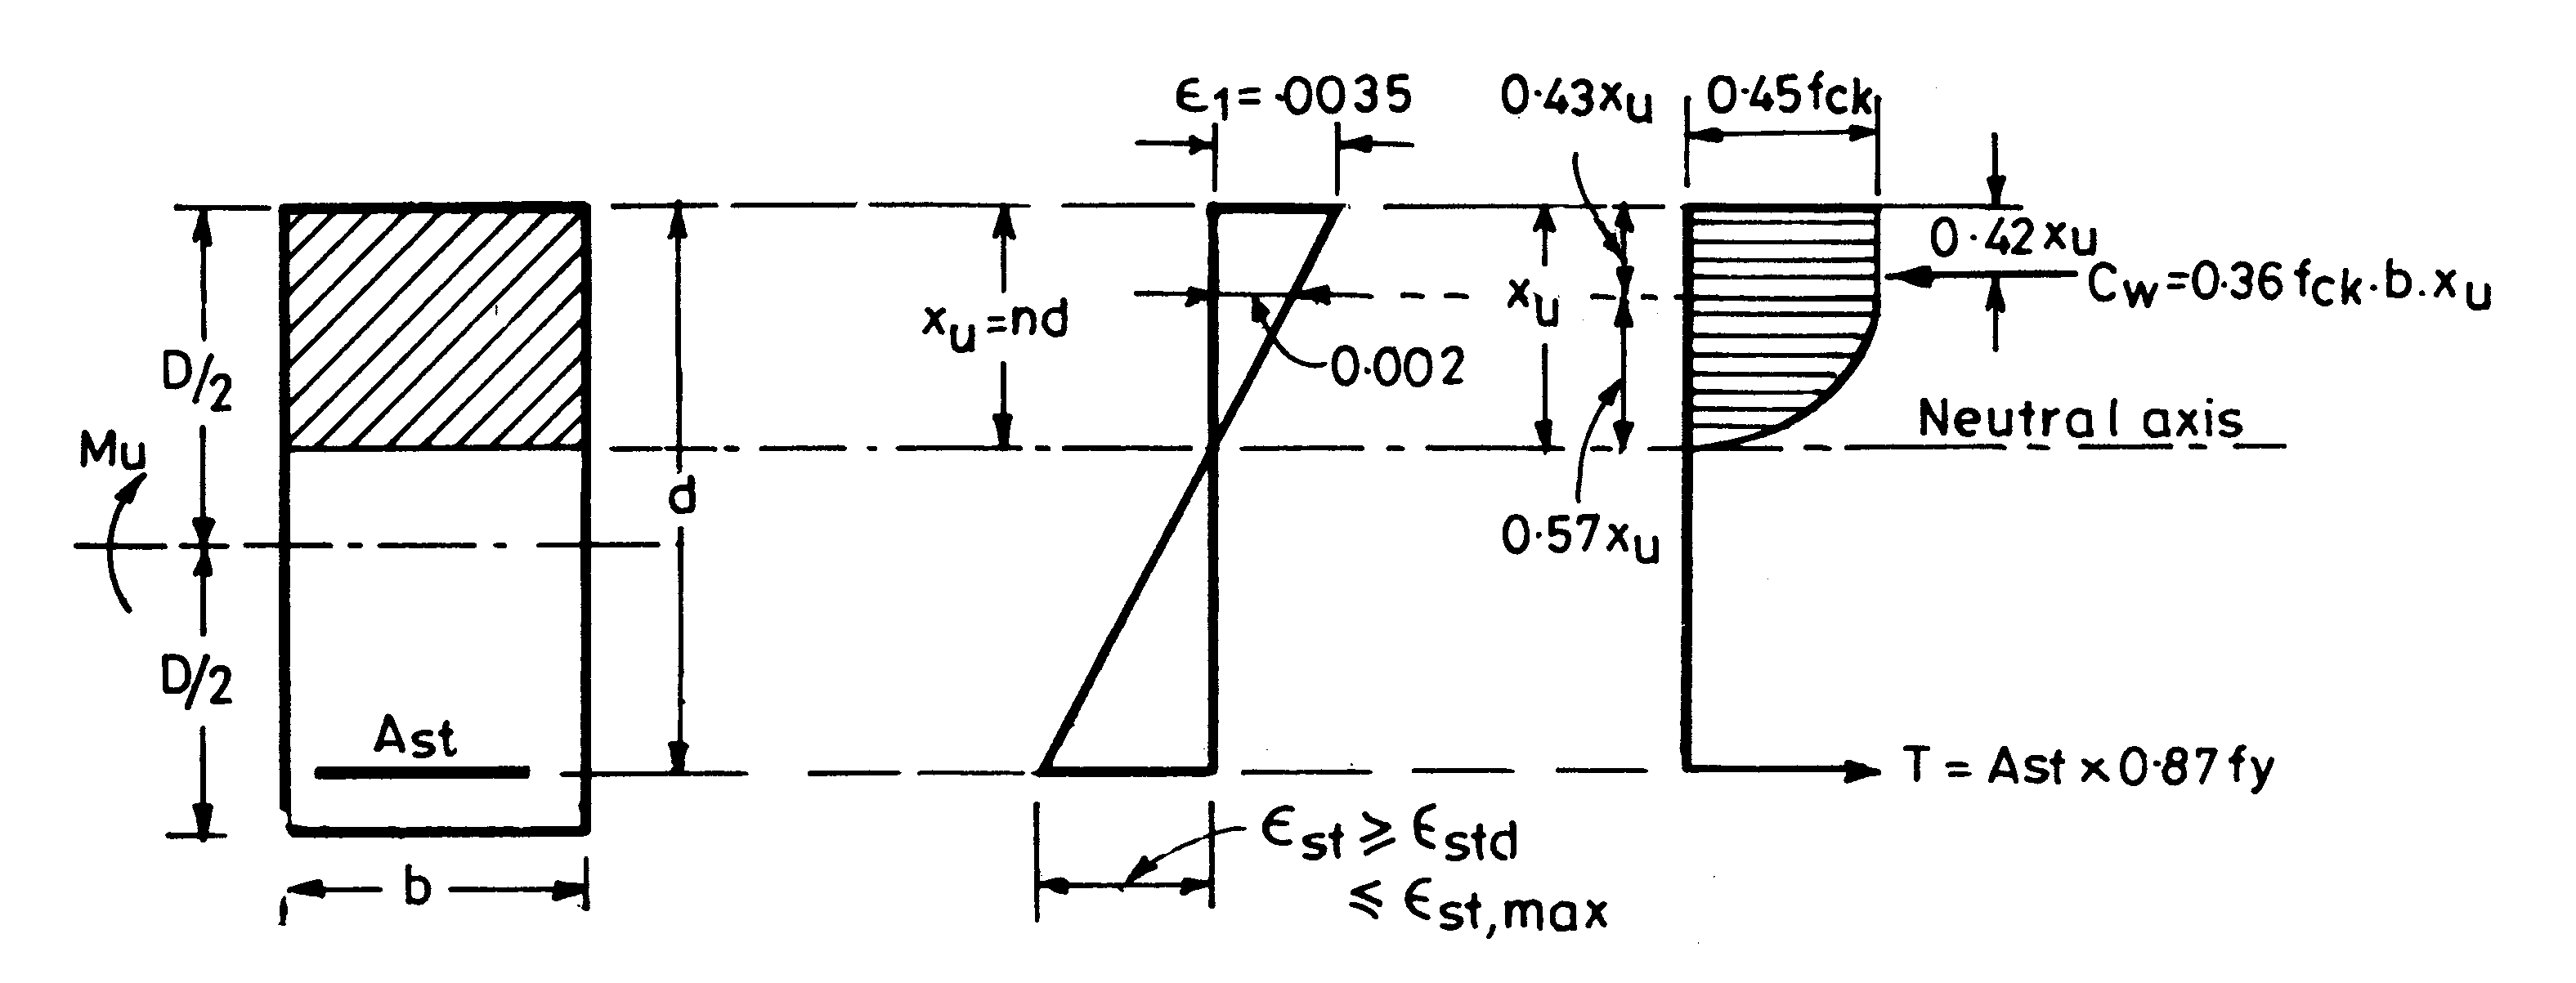
\includegraphics[width=0.8\textwidth]{images/ch2-1.png}
\caption{Singly reinforced rectangular section with concrete fully crushed at collapse.}
\label{Singly reinforced section 1}
\end{figure}
%---------------------------------------------------------------------------------------
\newpage
Equations \eqn \ref{Singly Reinforced}  and \eqn \ref{Reinforced Section}  give, on simplification,
\begin{equation}
\mu = 0.36n
\label{Concrete}
\end{equation}
\begin{equation}
k=\mu(1-0.42n)
\label{Crushed at collapse}
\end{equation}
These equations are the same as given by the Code in its Appendix G-1.1. The Code has,
however, not made clear that these equations do not apply for low values of n, When the tension
steel strain exceeds the maximum tension steel strain, for the simple reason that the Code
has made no stipulation in this regard. The Code has instead given the provision of the
minimum area of tension reinforcement,
$$\frac{A_s(min)}{bd} = \frac{0.85}{f_y}$$
which will greatly limit the tension steel strain and thereby restrict cracking and spalling of
concrete of tension zone.\\
When the position of neutral axis is such that O S xu S xu, min, the concrete compression
zone is subjected to only a part of the standard concrete stress diagram given by the Code and
the above expressions are not valid for this range. The conditions of equilibrium of the section
\fig \ref{Singly reinforced section}give on simplification,
\begin{figure}
\centering
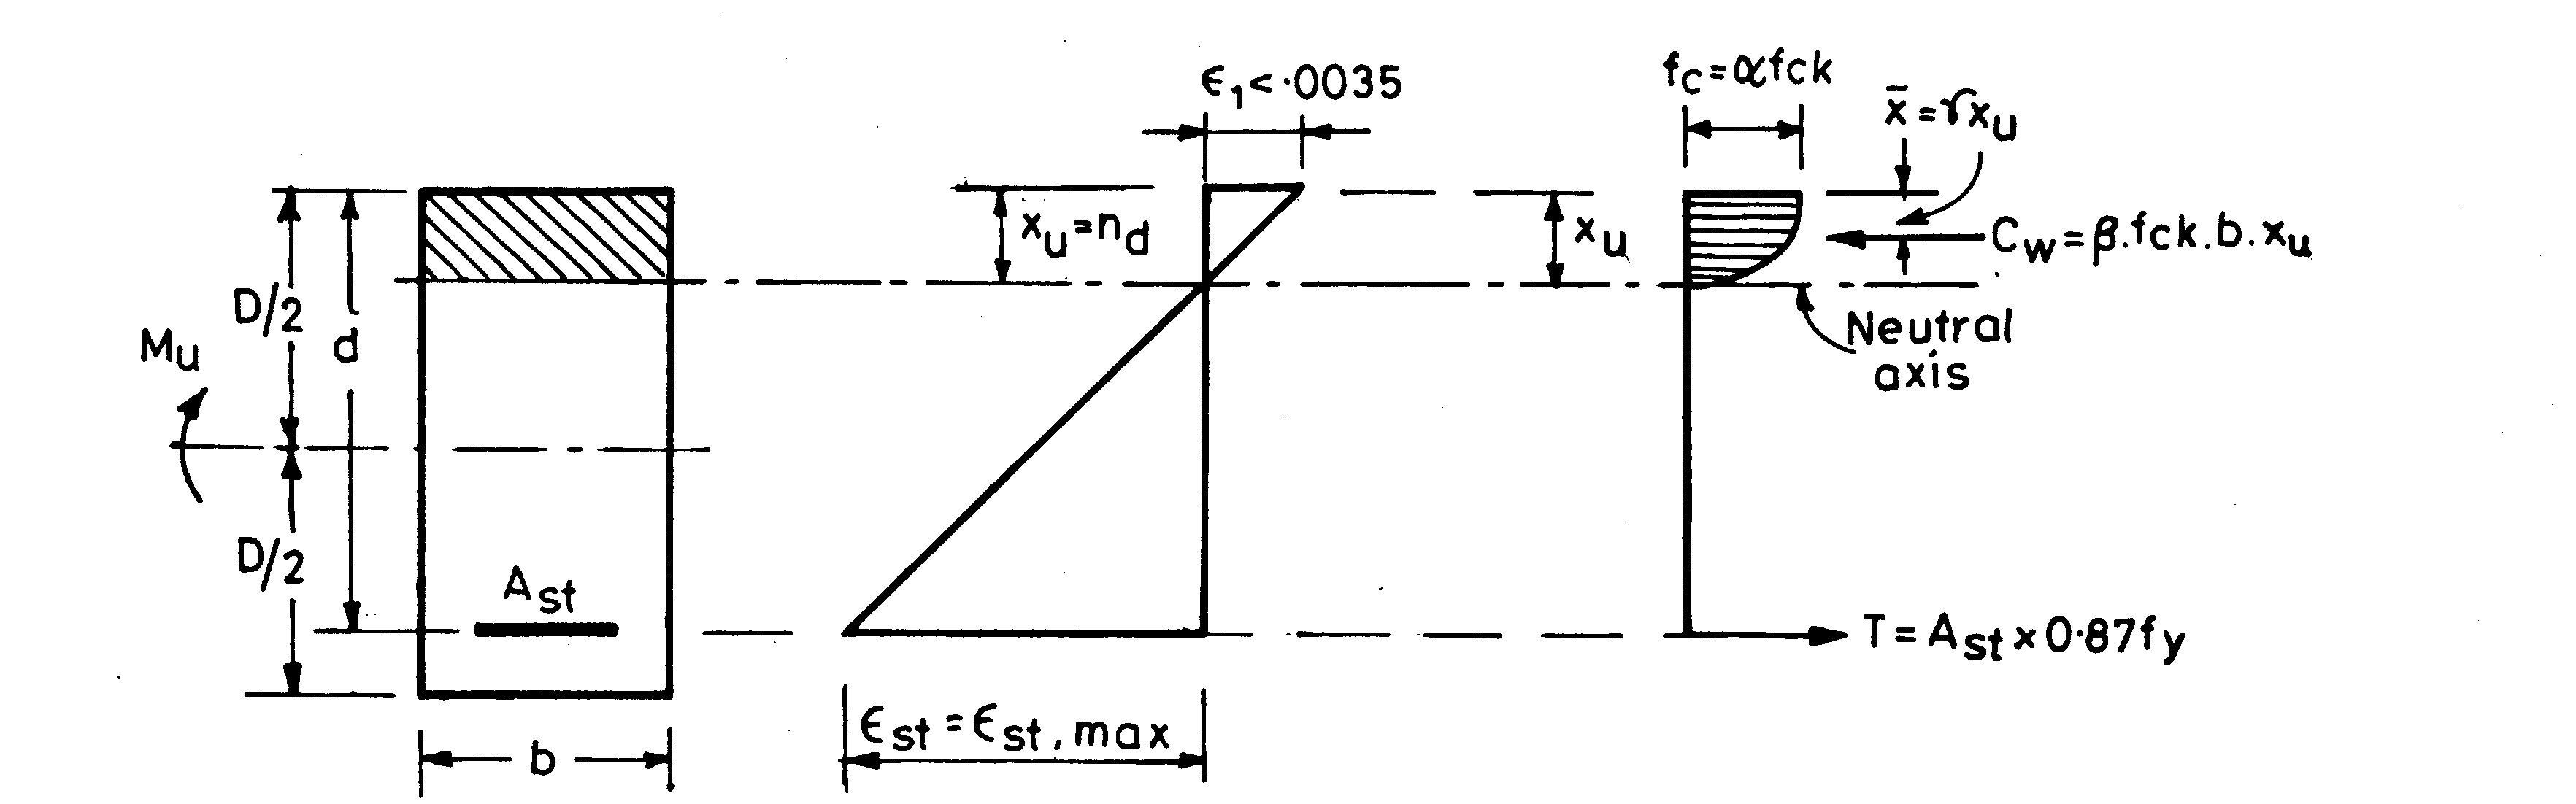
\includegraphics[width=0.8\textwidth]{images/ch2-2.png}
\caption{Singly reinforced rectangular section with concrete not fully crushed at collapse.}
\label{Singly reinforced section}
\end{figure}
\begin{figure}
\centering
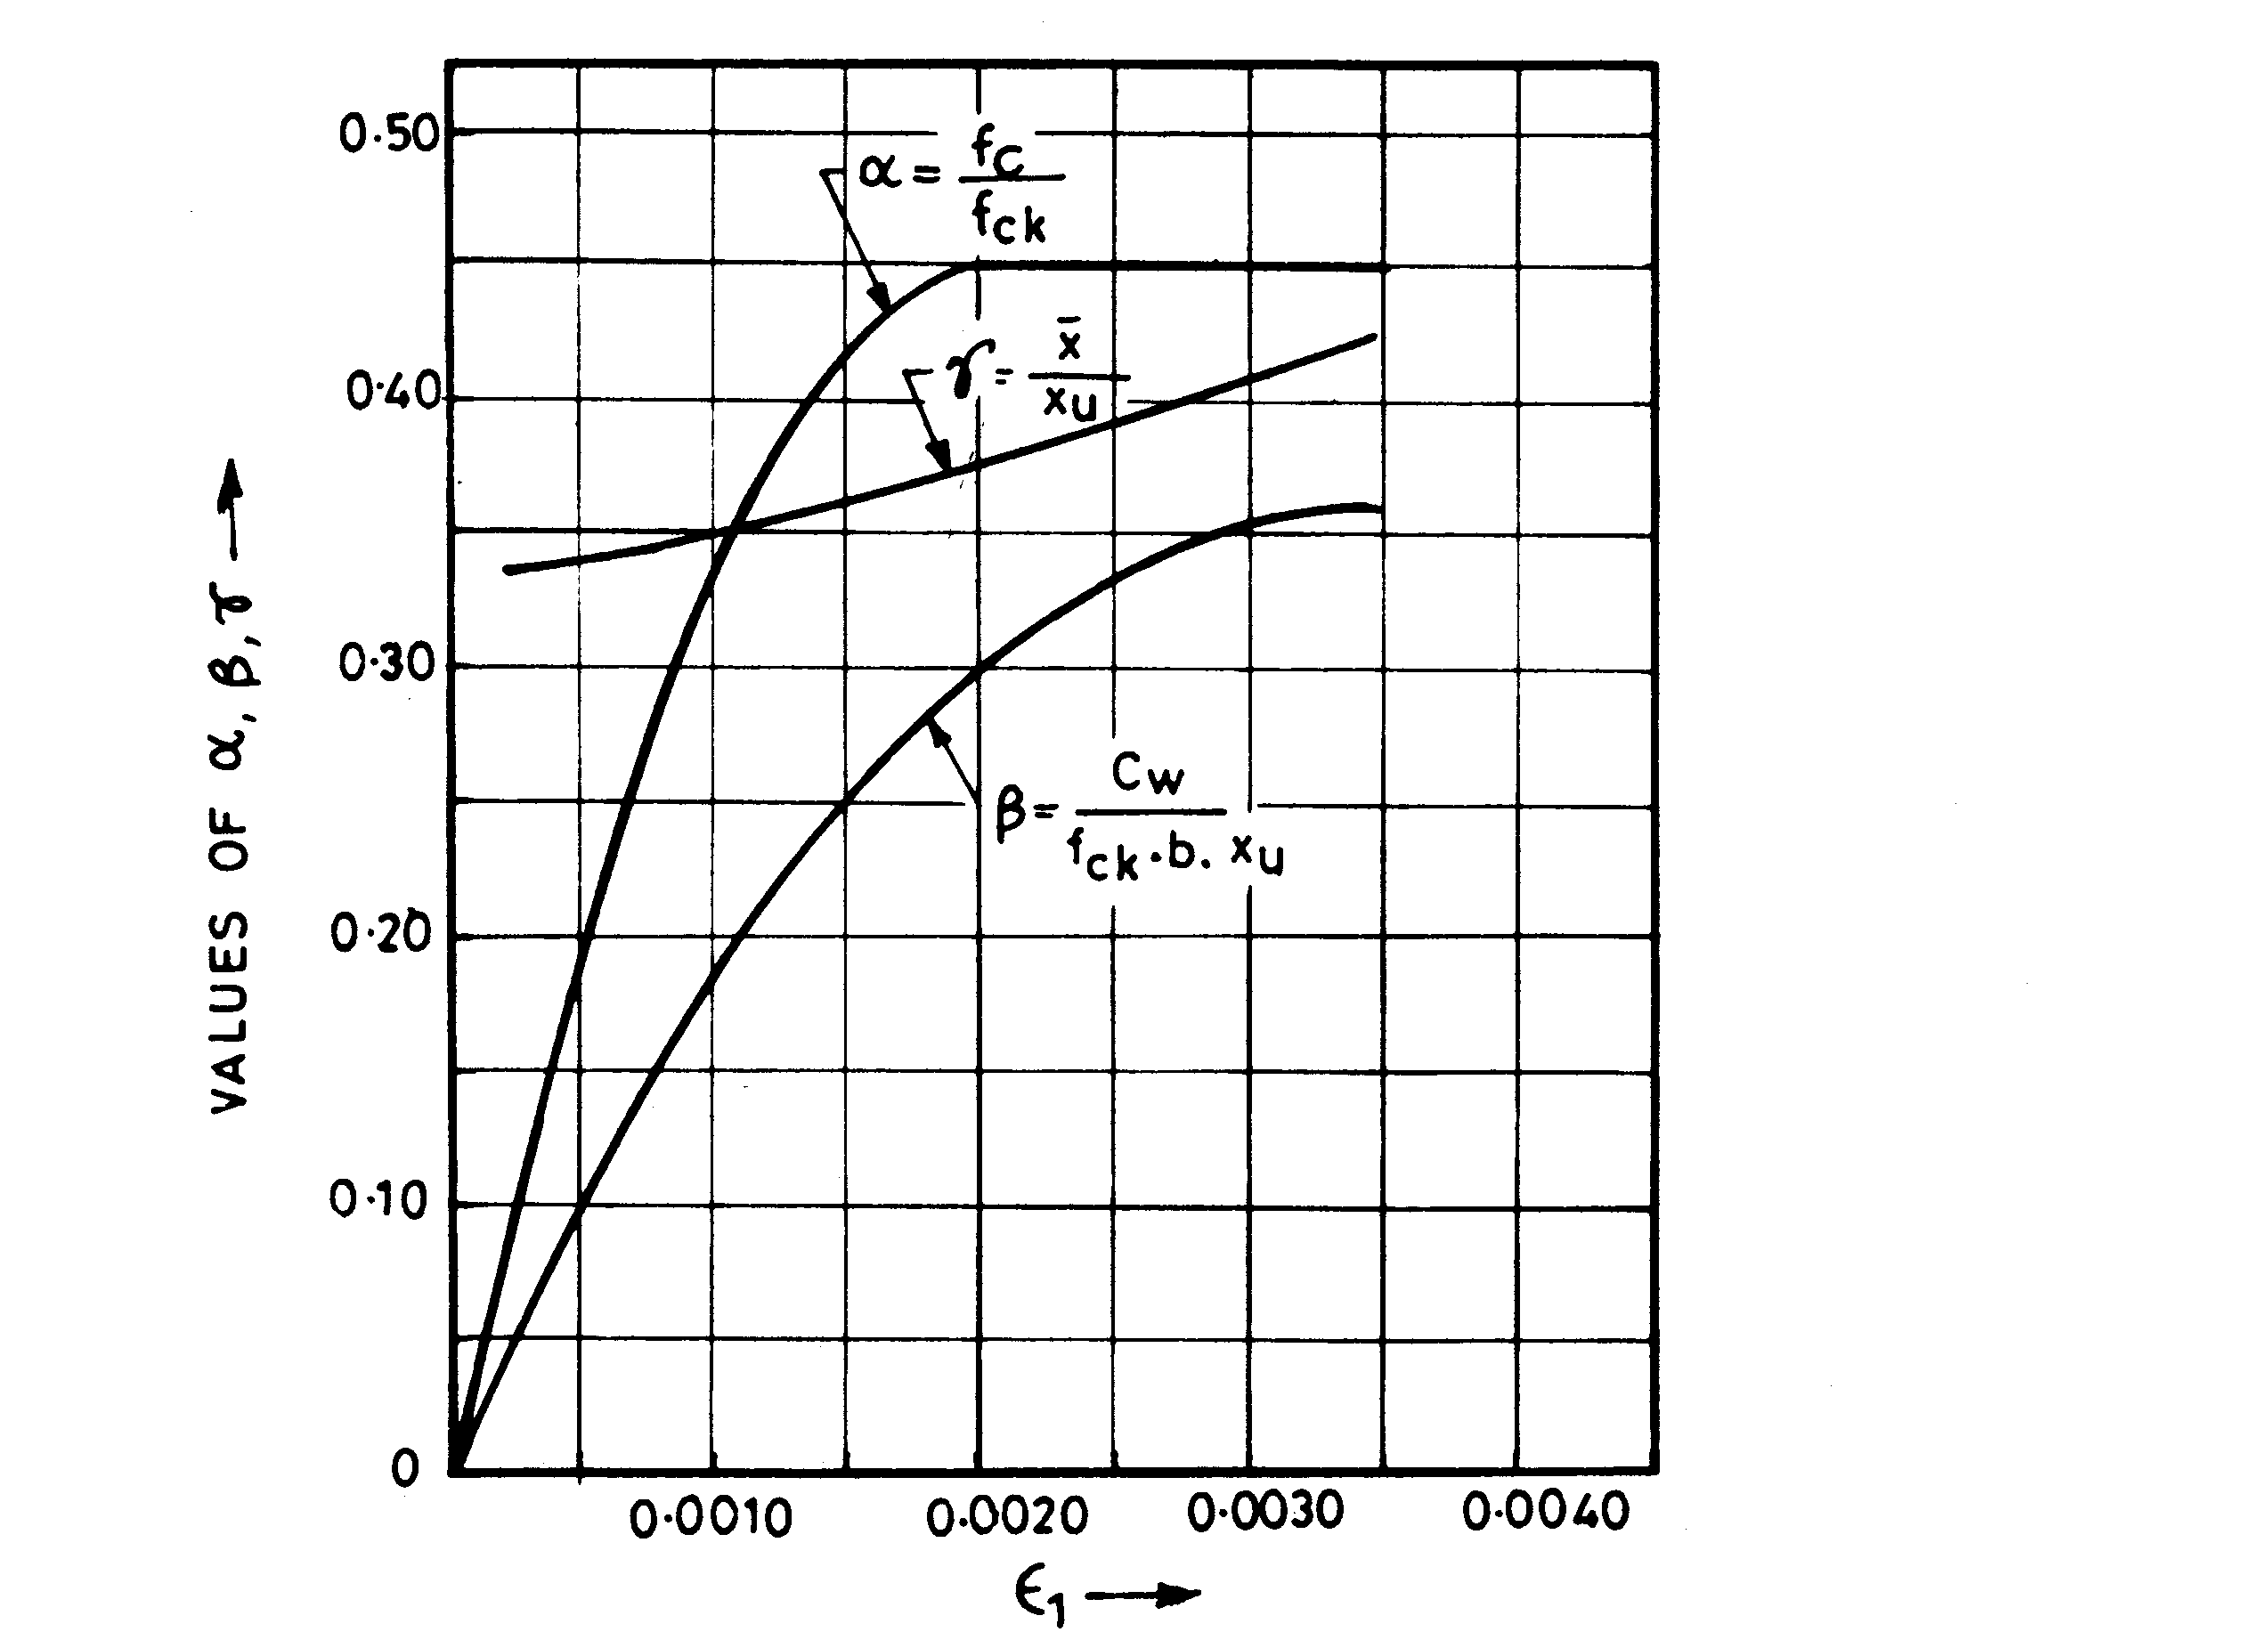
\includegraphics[width=0.8\textwidth]{images/ch2-3.png}
\caption{Values for non-dimensional parameters ${\alpha}$,${\beta}$ and ${\gamma}$ \fig \ref{Singly reinforced section}.}
\label{Values for parameters}
\end{figure}
%--------------------------------------------------------------------------------------------
\newpage
\begin{equation}
\mu=\beta.n
\label{non-dimensional}
\end{equation}
\begin{equation}
k=\mu(1-\gamma.n)
\label{parameters}
\end{equation}
where
\begin{equation}
\hspace{2cm} \beta = \frac{C_w}{f_ck\hspace{0.1cm}.\hspace{0.1cm}b\hspace{0.1cm}.\hspace{0.1cm}x_u}
\label{Beta value}
\end{equation}
\begin{equation}
\gamma = \frac{\bar{x}}{x_u}
\label{stress}
\end{equation}
The concrete stress at the extreme fibre of section \fig \ref{Singly reinforced section} is given by
\begin{equation}
f_c = \alpha.f_ck
\label{extreme fibre section}
\end{equation}
The non-dimensional parameters on $\alpha$, $\beta$, and $\gamma$ can be read from \fig \ref{Values for parameters}, which gives curves for
these parameters with respect to the concrete compression strain at the extreme fibre of section
(81) derived simply by rules of Geometry.


Equations \eqn \ref{non-dimensional}and \eqn \ref{parameters} apply when n $<$ $(n_{min})$ and Eqs. \eqn \ref{Concrete} and \eqn \ref{Crushed at collapse} apply when $(n_{min})$ ${\leq}$ n ${\leq}$ $(n_{max})$.
When n $>$ $(n_{max})$, the Code prescribes that n = $(n_{max})$ must be assumed for
ensuring ductility. With n =$(n_{max})$, equation \eqn \ref{Section4} gives the limiting moment of resistance
(M u, am) of singly reinforced rectangular section as,
\begin{equation}
M_{u,lim} = 0.36 n_{max}(1-0.42n_{max})\hspace{0.1cm}.\hspace{0.1cm}f_ck\hspace{0.1cm}.\hspace{0.1cm}bd^2
\label{Singly R Section}
\end{equation}
\section{Doubly Reinforced Rectangular Section}
When the applied moment $M_u$ is greater than the limiting moment of resistance $(M_{u,lim})$
of a given singly reinforced rectangular section, compression reinforcement is required to be
provided giving a doubly reinforced section. The equilibrium of the section \fig \ref{reinforced section} gives,
\begin{equation}
T = C_w + C_s
\label{Equillibrium of section}
\end{equation}
\begin{equation}
M_u = C_w(d-0.42x_{u,max}) + C_s(d-d ')
\label{EOSII}
\end{equation}

\begin{figure}
\centering
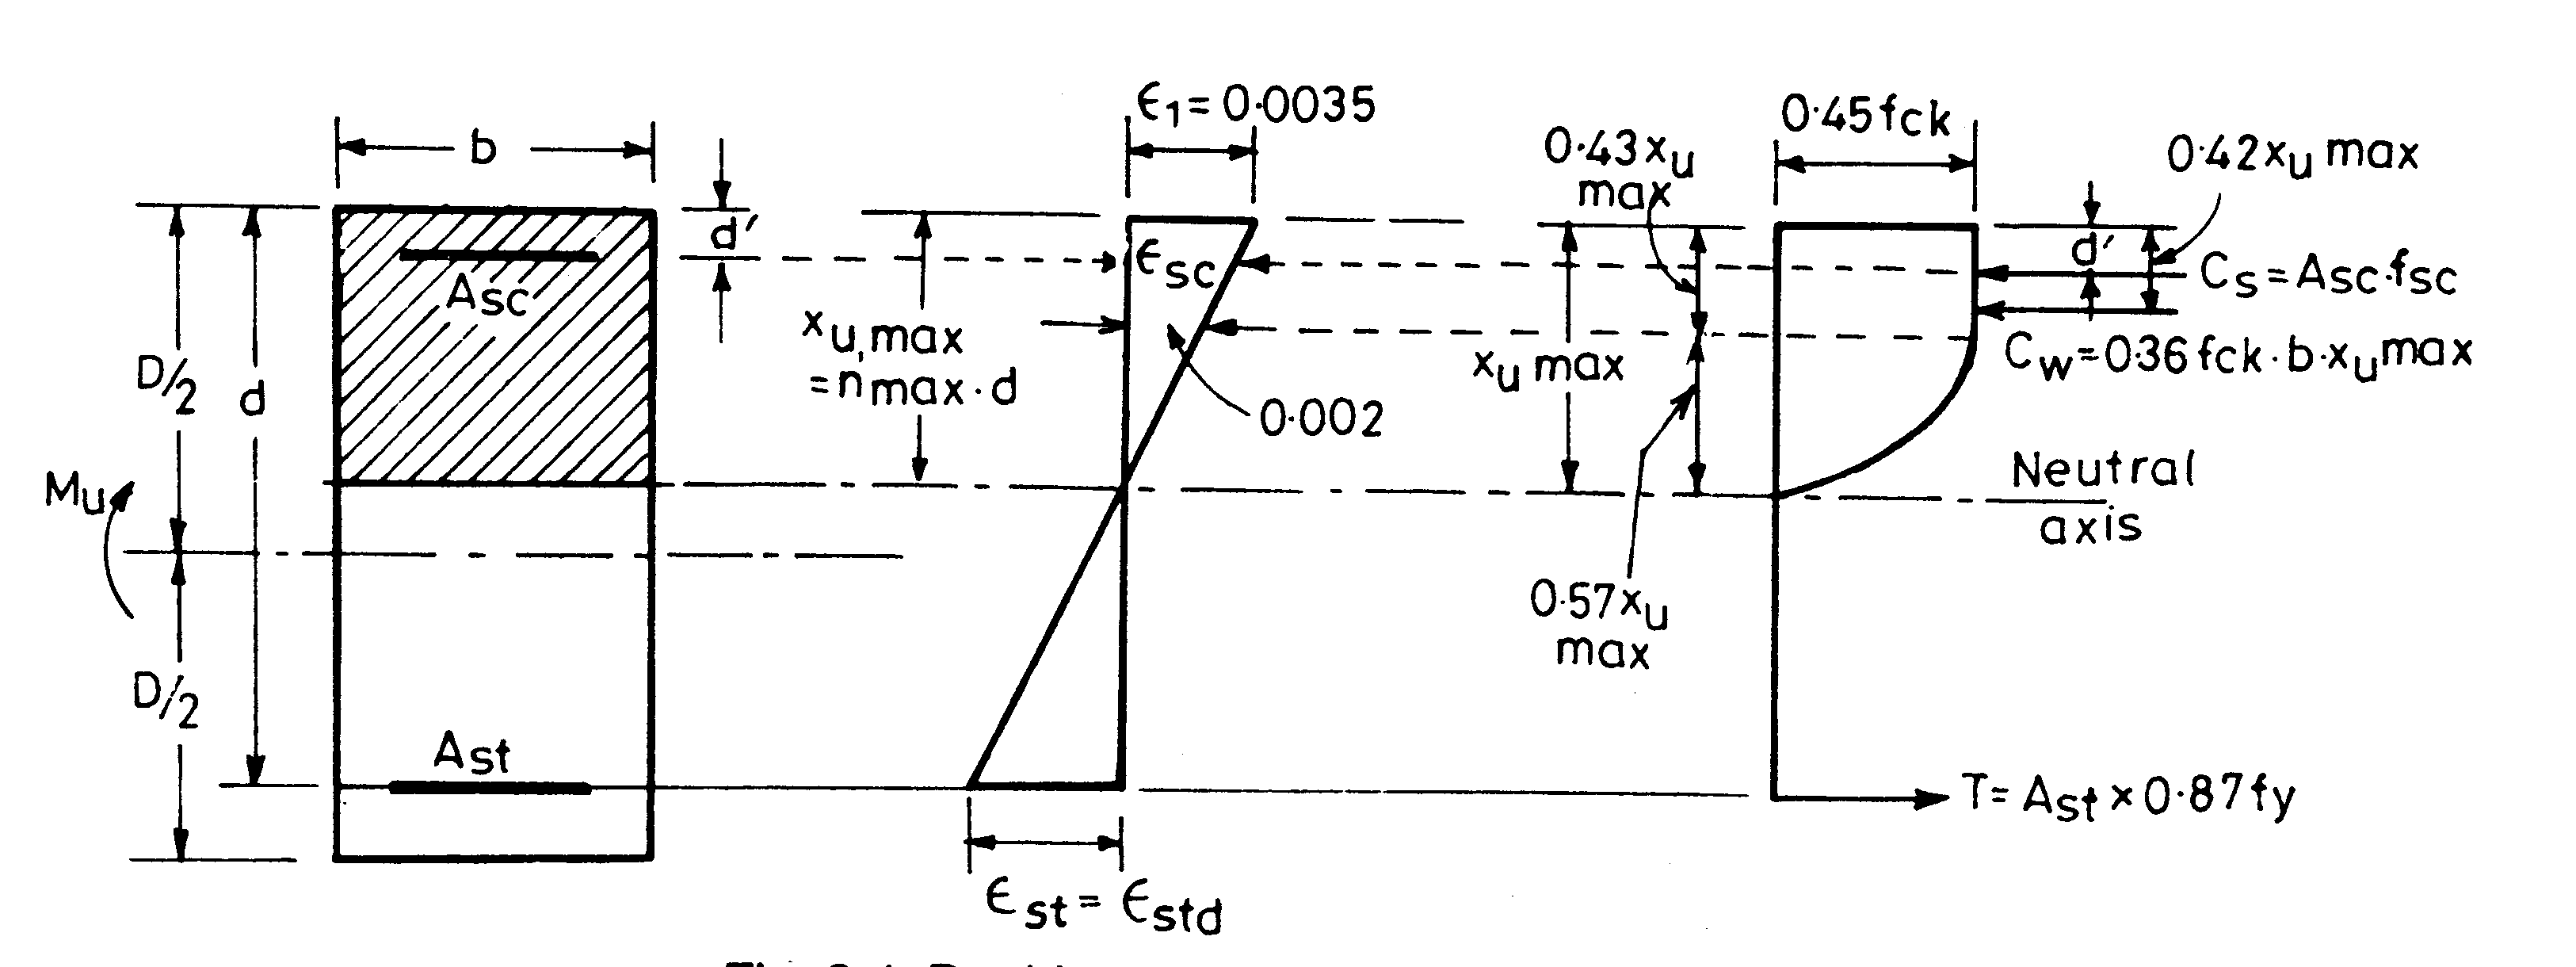
\includegraphics[width=0.8\textwidth]{images/ch2-4.png}
\caption{Doubly reinforced rectangular section.}
\label{reinforced section}
\end{figure}
Introducing an additional non-dimensional parameter,
$$\mu' = \frac{A_{sc}}{bd} \times \frac{f_{sc}}{f_{ck}}$$
These equations give, on simplification,
\begin{equation}
\mu=0.36n_{max} + \mu'
\label{Additional parameter}
\end{equation}
%-----------------------------------------------------------------------------------------
\newpage
\begin{equation}
k=0.36n_{max}(1-0.42n_{max}) + \mu'(1-\frac{d'}{d})
\label{APII}
\end{equation}
Value of $(f_{sc})$ is to be read from \fig 23 of the Code corresponding to compression steel strain
($\varepsilon_{sc}$), which is given by \fig \ref{Doubly reinforced rectangular section.},

\begin{equation}
\varepsilon_{sc} = 0.0035(1-\frac{1}{n_{max}}.\frac{d'}{d})
\label{Compression steel strain}
\end{equation}
\section{Design Charts}
Equations \eqn \ref{Concrete} to \eqn \ref{parameters} are used to develop charts for singly reinforced rectangular
sections. For an assumed value of n, relevant equations from those given above are used. to
give values for k and $\mu$, which are plotted to give \chartm 2.1 and 2.2, one each for steel types
Fe 250 and Fe 415. For doubly reinforced sections, equations \eqn \ref{Additional parameter} and \eqn \ref{APII} are used to get
values for $\mu$ and k for an assumed value of $\mu’$ and d'/d. These give a series of straight lines for
k, which depend on d'/d, while the straight line for$\mu’$is independent of d'/d . \chartm 2.1 and 2.2
give all these curves with Y-Y axis representing n or $\mu’$, where n applies for singly reinforced
sections and $\mu’$ for doubly reinforced sections. Values for$(f_{sc})$ are given against values of d'/d in
each chart for ready use. There is an advantage in plotting curves for singly and doubly
reinforced sections on the same co-ordinate axes, in that, the (capacity of a singly reinforced
section need not be specially checked when the applied moment is greater than it. Use of design
charts is illustrated by the following numerical examples.
\section{Numerical Examples}
\begin{example}
 Singly Reinforced Rectangular Section (Design)

\given 
b = 30 cm, $(f_{ck})$ = 1.5 $\knpcs$

 D = 60 cm, $f_y$ = 41.5 $\knpcs$

d = 56.25 cm, $M_u$  = 170 $\knm$

This example is taken from Design Aids$^{8}$ (Page 11).

\required$(A_{st})$

\solution
$$k= \frac{170 \times 100}{1.5 \times 30 \times (56.25)^2} =0.119$$
Chart 2.2 gives,
$$n=0.40$$, 
$$\mu=0.145$$
$$A_{st}=\frac{0.145 \times 30 \times 56.25 \times 1.50}{0.87 \times 41.5} = 10.17 cm^2$$
\end{example}

\begin{example} Singly Reinforced Rectangular Section (Investigation).

\given Same as Ex.2.1 with $(A_{st})$= 6.40 cm$^{2}$

\required $(M_{u})$

\solution
$$\mu=\frac{6.40 \times 0.87 \times 41.5}{30 \times 56.25 \times 1.5} =0.09$$
Chart 2.2 gives,
$$n=0.245, \mu=0.0775$$
$$M_{u}=0.0775 \times 1.50 \times 30 \times (56.25^2)/100= 110\knm.$$
\end{example}
%------------------------------------------------------------------------------
\newpage
\begin{figure}
\centering
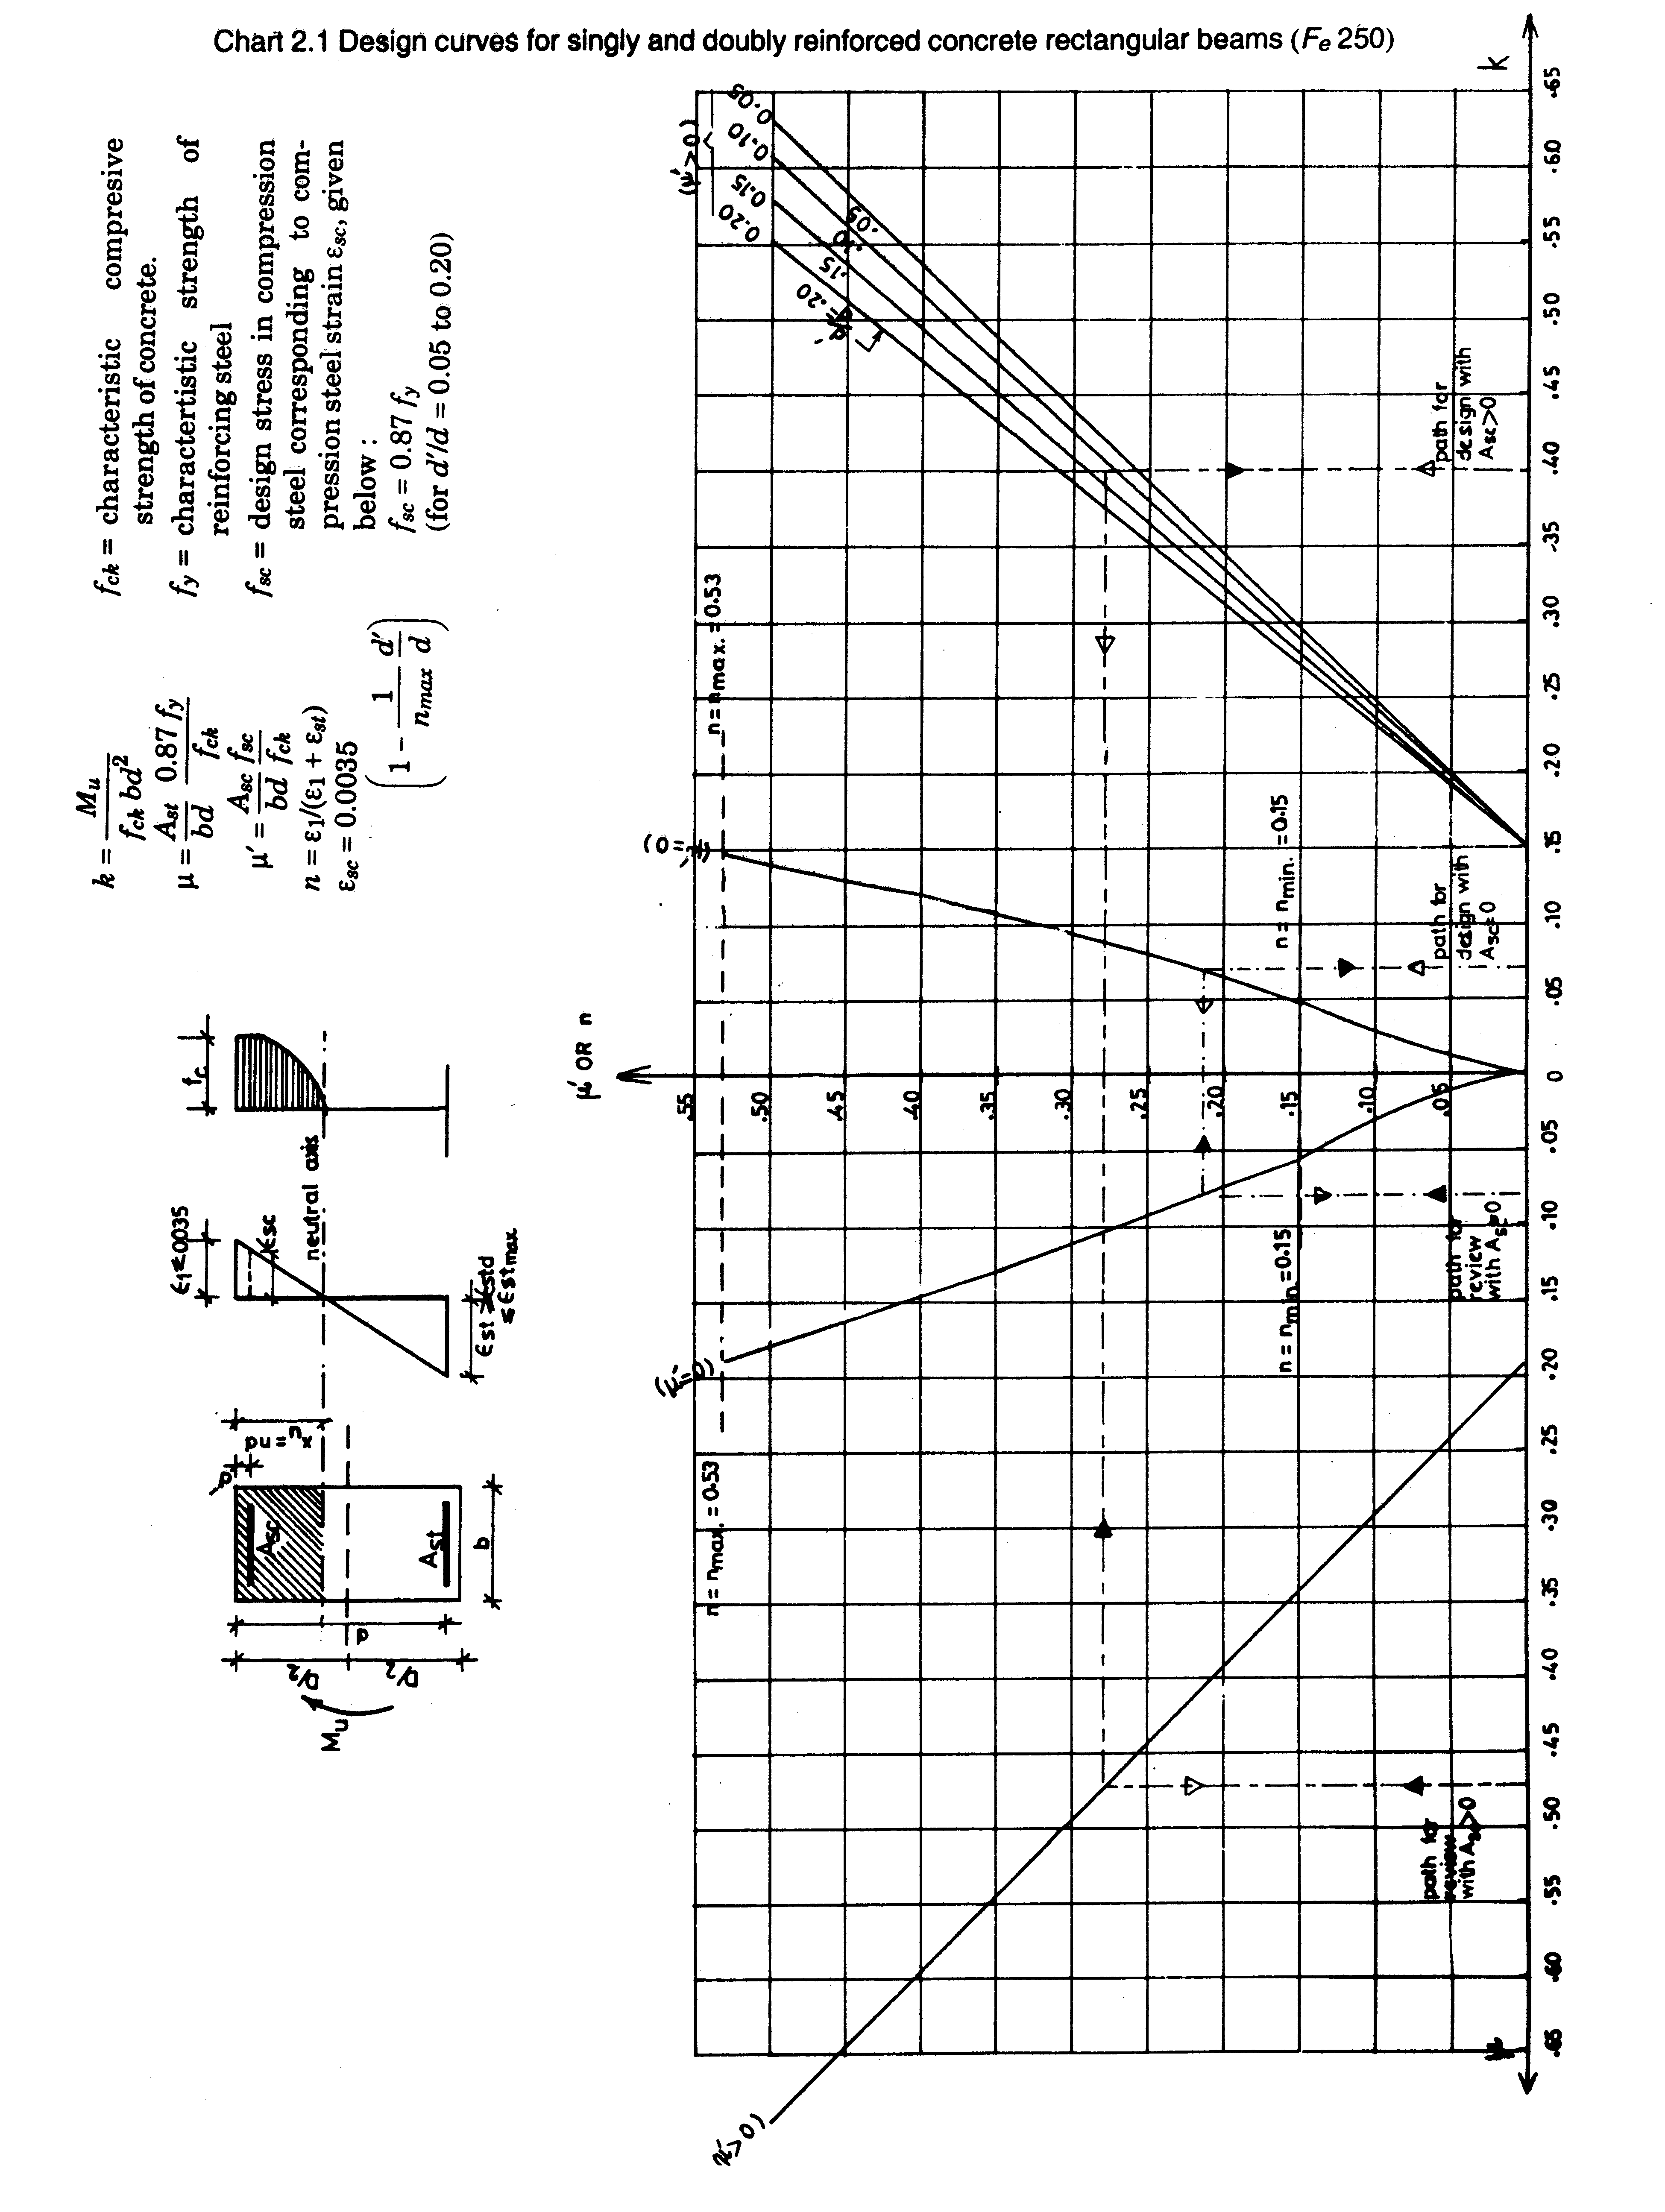
\includegraphics[width=0.95\textwidth]{images/ch2-5.png}
\caption{}
\label{fig:Values for parameters}
\end{figure}
%-------------------------------------------------------------------------------
\newpage
\begin{figure}
\centering
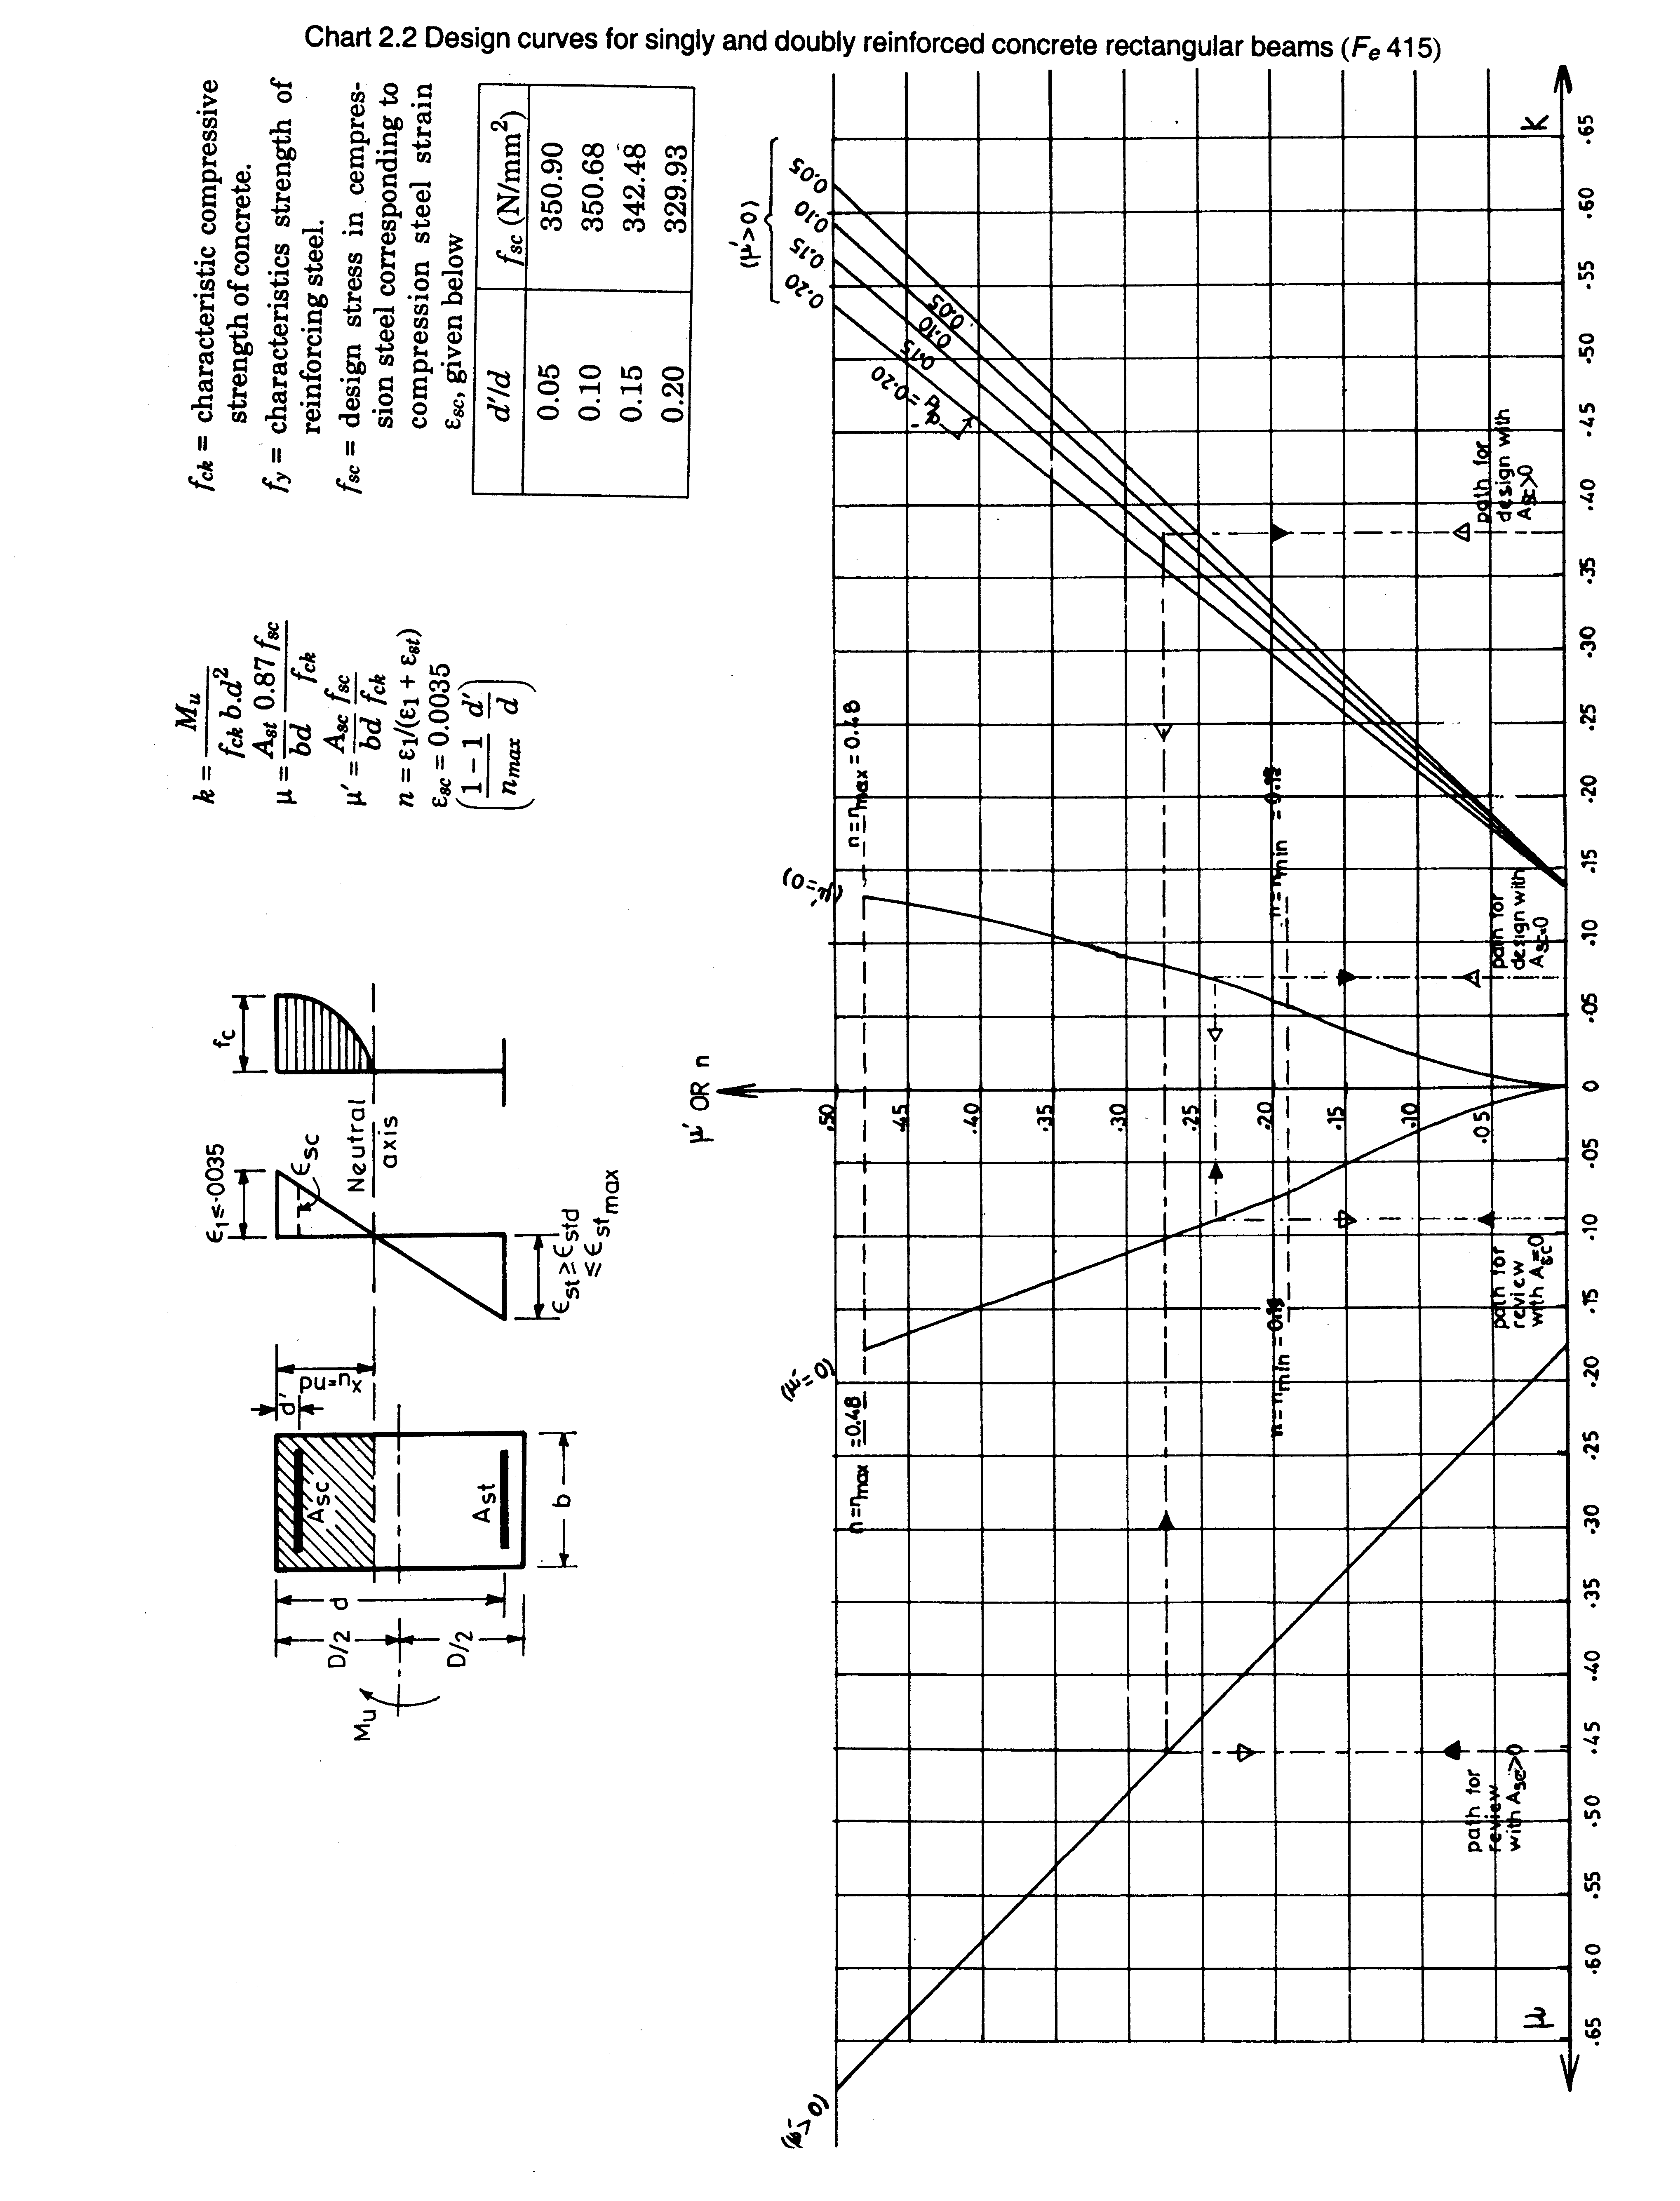
\includegraphics[width=0.95\textwidth]{images/ch2-6.png}
\caption{}
\label{Values for parameters}
\end{figure}
%------------------------------------------------------------------------------------
\newpage
\begin{example} Doubly Reinforced Rectangular Section (Design).

\given Same as in Ex. 2.1 but with $(M_{u})$= 320 kNm and d’ = 3.75 cm. This example is taken
from Design Aids$^{8}$(Page 13).

\required $(A_{st})$, $(A_{sc})$
\solution
$$k=\frac{320 \times 100}{1.50 \times 30 \times (56.25)^2}=0.225$$
Chart 2.2 gives for
$$\frac{d'}{d}=\frac{3.75}{56.25}=0.067$$ 
$$\mu'=0.0925.\mu=0.265$$
$$A_{st}=\frac{0.265 \times 30\times 56.25 \times 1.50}{0.87 \times 41.5}=18.58cm^2$$
For
$$\frac{d'}{d}=0.067$$
Chart 2.2 gives by interpolation
$$f_{sc}=35.48\knpcs$$
$$A_{sc}=\frac{0.0925 \times 30 \times 56.25 \times 1.50}{35.48}=6.60cm^2$$
\end{example}


\begin{example} Doubly Reinforced Rectangular Section (Implementation).

\given  Same as in Ex. 2.1 but with $(A_{sc})$=4.0cm$^{2}$
$$A_{st}=18.0cm^2 \hspace{0.1cm}and\hspace{0.1cm} d'=3.75$$
\required $M_u$

\solution For
$$\frac{d'}{d}=0.067$$ \chartm 2.2 gives,
$$f_{sc}=35.48\knpcs$$
$$\mu'=\frac{4.0 \times 35.48}{30 \times 56.25 \times 1.50}=0.056$$
Chart 2.2 gives for $\frac{d'}{d}$=0.067
$$k=0.19$$
$$M_u= 0.19 \times 1.50 \times 30 \times (56.25)^2/100=270\knm.$$ 
A check on the adequacy of tension steel area is further required. For $\mu'$ = 0.056, \chartm 2.2
gives
$$\mu=0.23$$
$$A_{st}(required)=\frac{0.23 \times 30 \times 56.25 \times 1.50}{0.87 \times 41.5}=16.12cm^2$$
which is less than the provided $(A_{sc})$= 18.0 cm$^{2}$

The capacity of the given section is, therefore, correctly computed to be 270 $\knm$.
\end{example}
%-----------------------------------------------------------------------------------------
\newpage
\section{Conclusion}
Design charts have been furnished for singly and doubly reinforced concrete rectangular
beams which are independent of concrete quality and are based on non-dimensional
parameters. These charts are quite concise and incorporate the modifications necessary for
low values of n. Further, these charts can be used with equal ease for design as well as
investigation of a given singly or doubly reinforced rectangular section.





